\chapter{Detalles de implementación}\label{cap:implementation_details}

Con el objetivo de garantizar que el lector esté más acorde con la tecnología usada para la implementación, las razones de esa elección, la forma de desplegar el sistema y demás aspectos relacionados con la parte tecnológica se expone esta capítulo.

A día de hoy se cuenta con muchas herramientas para desarrollar un software de este tipo. En esta ocasión se escogió una tecnología que ha alcanzado bastante auge en los últimos años. En las secciones siguientes se hará alusión a la misma así como al lenguaje empleado para el desarrollo.

\section{Tecnologías}
Para este proyecto se utilizó el lenguaje TypeScript, auxiliándonos de NestJS (framework de NodeJS).

\label{lenguage}
\cite{wiki_ts}
TypeScript(TS) es un lenguaje de programación libre y de código abierto desarrollado y mantenido por Microsoft. Es un superconjunto de JavaScript(JS), que esencialmente añade tipos estáticos y objetos basados en clases. Anders Hejlsberg, diseñador de C\# y creador de Delphi y Turbo Pascal, se considera el desarrollador del lenguaje. TS es usado para desarrollar aplicaciones JS que se ejecutarán tanto en el lado del cliente como del servidor. El lenguaje extiende la sintaxis de JS, por tanto cualquier código JS existente debería  funcionar sin problemas. Está pensado para grandes proyectos, los cuáles a través de un compilador de TS se traducen a código JS original. TS soporta ficheros de definición que contengan información sobre los tipos de librerías JS existentes; esto permite a otros programas usar los valores definidos en los ficheros como si fueran entidades TS de tipado estático. El compilador de TS está escrito asimismo en TS. 

El lenguaje fue publicado en octubre de 2012 , después de dos años de desarrollo por parte de la compañía y desde esa fecha ha tenido en general, buena aceptación por parte de todos, lo que le mereció el mérito en 2020 como segundo lenguaje de programción más amado según la encuesta de Stack Overflow\cite{stack_overflow} 2020 Develop Survey.

\cite{nestjs_doc}
NestJS es un framework para construir eficientes y escalables aplicaciones del lado del servidor utilizando NodeJS. Posee soporte tanto para JS como para TS y combina elementos de Programación Orientada a Objetos (OOP, por sus siglas en inglés), Programación Funcional y Programación Funcional Reactiva. Nest posee un robusto framework HTTP basado en \textit{Express} (definido por defecto) y opcionalmente se puede configurar además el uso \textit{Fastify} como alternativa a \textit{Express}.

Ofrece un nivel de abstracción superior al que normalmente encontramos en los demás frameworks de Node(Express/Fastify), pero también expone sus APIs directamente al desarrollador. Esto le ofrece a los programadores la libertad de emplear la mayoría de las aplicaciones de 3$^{ros}$ desarrolladas para esos otros ambientes.

En los últimos años gracias a Node, ha supuesto un cambio sustancial en el desarrollo de aplicaciones del lado del servidor, pero, por otra parte y a pesar de las bondades que ofrece, aún no presenta una solución efectiva al problema de arquitectura. 

Nest se presenta como solución a esto, ya que posee una estructura que induce desde el principio a la utilización de patrones arquitectónicos. La arquitectura de Nest es inspirada en Angular.

Fue desarrollado por Kamil Mysliwiec, desarrollador de Google; el lanzamiento de su versión 9 se realizó el 8 de Julio de 2022.


\section{Arquitectura}

El  sistema presentado encierra una gran lógica de negocio y encontrar una forma aceptada de representar el mismo puede resultar, en muchos casos, de gran dificultad.

Para asegurar el correcto diseño de la aplicación, su posible extensión y adición de nuevas features (características), se hizo neceario utilizar una arquitectura, quizá un poco compleja, pero que permitiera enfocar todos los casos de uso que puedan surgir. 

El diseño guiado por dominio (DDD por sus siglas en inglés) es un enfoque para el desarrollo de software con necesidades complejas, mediante una profunda conexión de la implementación con los conceptos del modelo y núcleo del negocio.\cite{ddd_wiki} 

Para el software que nos envuelve se emplea una arquitectura por capas (Layered Architecture), centrada en DDD. Este enfoque es, sin lugar a dudas, una de los más empleados hoy en día. Impone una jerarquía y un acceso restringido a cada una de las estructuras del código; dígase: dominio, aplicación, infraestructura y presentación; las cuáles se encargan de la separación de las responsabilidades, y por tanto de la gestión de elementos específicos.

\begin{itemize}
	\item Dominio: Gestiona todo lo referente a la lógica que involucra las entidades descritas en las secciones previas (\ref{sec:entities}). Es la capa fundamental dentro de DDD.
	\item Aplicación: Se encarga de manejar todos los casos de uso que relacionados con cada entidad. A modo de ejemplo, todo sistema cuenta con cuatro casos de uso básicos: crear, leer, eliminar y editar.
	\item Infraestructura: Maneja todo lo relacionado con el acceso a datos. Contiene los repositorios y por tanto define una especie de envoltura (wrapper) que evita que se acceda directamente a la base de datos.
	\item Presentación: Se encarga de exponer todos los puntos de acceso a la API (Application Program Interface) y de gestionar  los consumidores (consumers), que tienen la responsabilidad de la gestión de eventos internos y externos al sistema.
\end{itemize}

\begin{figure}[h]
	\centering
	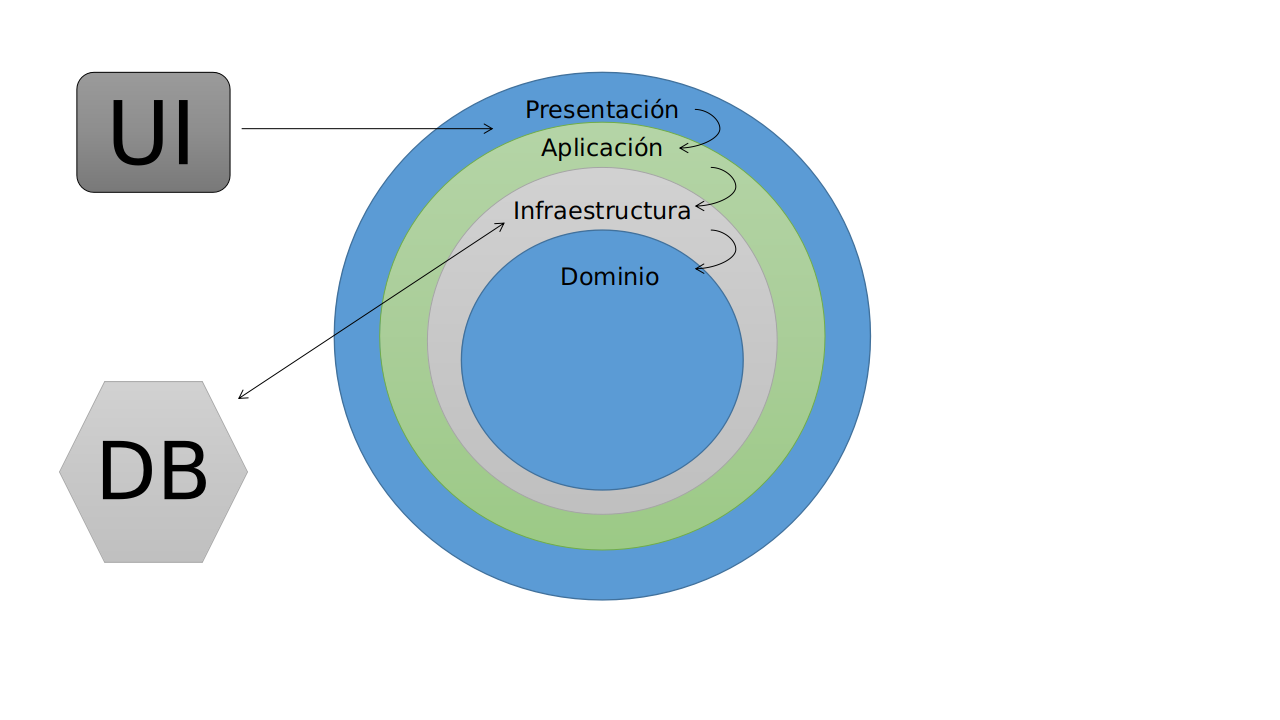
\includegraphics[width=0.75\linewidth]{images/Chapter 3/DDD}
	\caption{Domain Driven Design}
	\label{fig:ddd}
\end{figure}


Los principios \textit{SOLID} \cite{solid_medium} abordados por Robert C. Martin (autor de diversos libros como Clean Code y Clean Arquitecture) se interaron seguir a través de toda la implementación.


\section{Aplicación visual}

La idea detrás de la aplicación visual surge inspirada en un sistema desarrollado hace un par de años dentro de la facultad por un grupo de estudiantes y que se presentó como proyecto a la jornada científica de ese curso. \cite{horarios_fac}

Se ofrece un sistema desarrollado en VueJS y que pretende seguir las buenas prácticas de desarrollo de frontend. Está escrito en JavaScript. El sistema posee un conjunto de vistas dedicadas a manejar todas las tareas administrativas referentes al software; dígase: creación de profesores, grupos, semestres, asignaturas y demás cuestiones referentes al centro educacional. Solamente para el usuario con los permisos adecuados están habilitadas tales características, es decir, el usuario administrador es el único que puede realizar modificaciones internas dentro del sistema.

En la página principal se definen 5 tipos de filtros que hacen posible una rápida interacción. Estos filtros se presentan útiles en un gran número de escenarios. Se muestra además, en la misma página, la opción de descargar el horario, la cual esta habilitada para cualquier tipo de usuarios. El número que se presenta en la parte superior izquierda es referente a la felicidad del sistema, aspecto que fue abordado en las secciones previas a este capítulo. (\ref{sec:happiness})

En la visualización general del horario, cada grupo posee un color específico para que se haga más sencilla su lectura, el color es posible definirlo por el administrador del sistema a la hora de la creación del grupo, luego todos los turnos de clase que se asocien al mismo, se mostrarán de ese color.

\begin{figure}[h!]
	\centering
	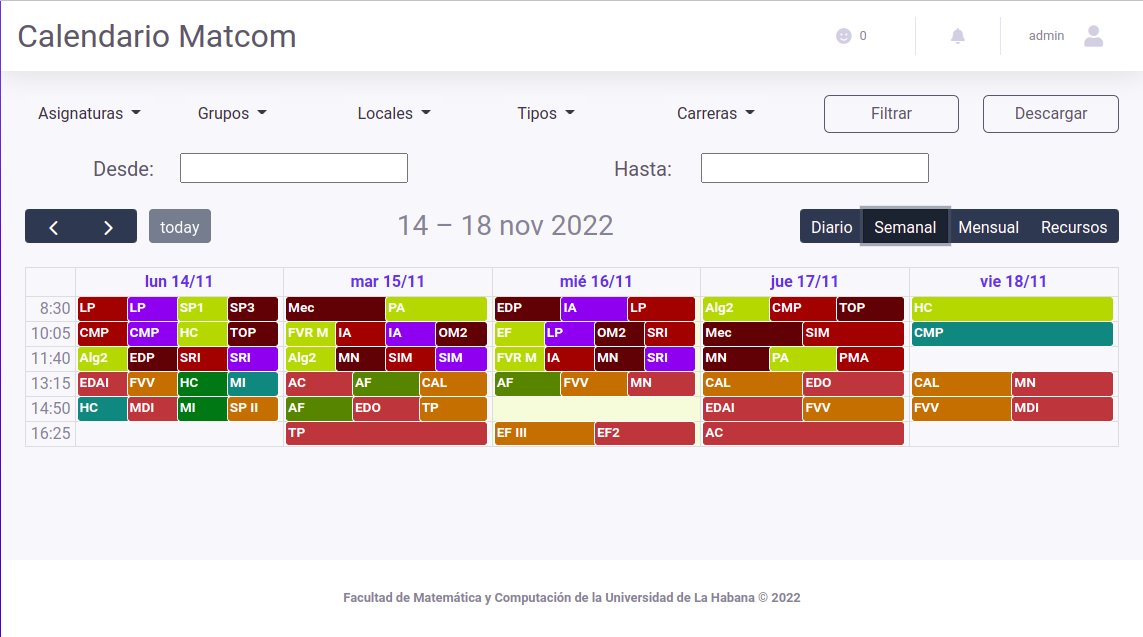
\includegraphics[width=0.95\linewidth]{images/Chapter 3/home}
	\caption{Vista por defecto del sistema.}
	\label{fig:home}
\end{figure}



En el manejo de la interfaz visual quizá resulte un poco llamativo para el administrador del sistema; que es el que tiene acceso a esas vistas; la creación, modificación y eliminación en serie que se muestra en cada \textit{modal} referente a los turnos de clases.  Este aspecto fue abordado con anterioridad, pero la acción que realiza es modificar todos los turnos que posean las mismas características del turno actual, es decir, que repitan el ciclo del horario para él.

Para cada turno visualizado es válido además modificarle la duración del mismo, esto se logra modificando el \textit{size} de este dentro del horario. Realizar esta acción es justo como modificarle el \textit{size} a cualquier otra ventana del sistema, lo que en esta ocasión es a la caja que describe el turno.

Haciendo clic encima del turno se obtine además una descripción detallada del mismo, así como las opciones para la edición y eliminación múltiple.

La vista de distribución por locales llama la atención y se presenta de gran importancia a la hora de considerar la usabilidad de la aplicación.

\begin{figure}[h!]
	\centering
	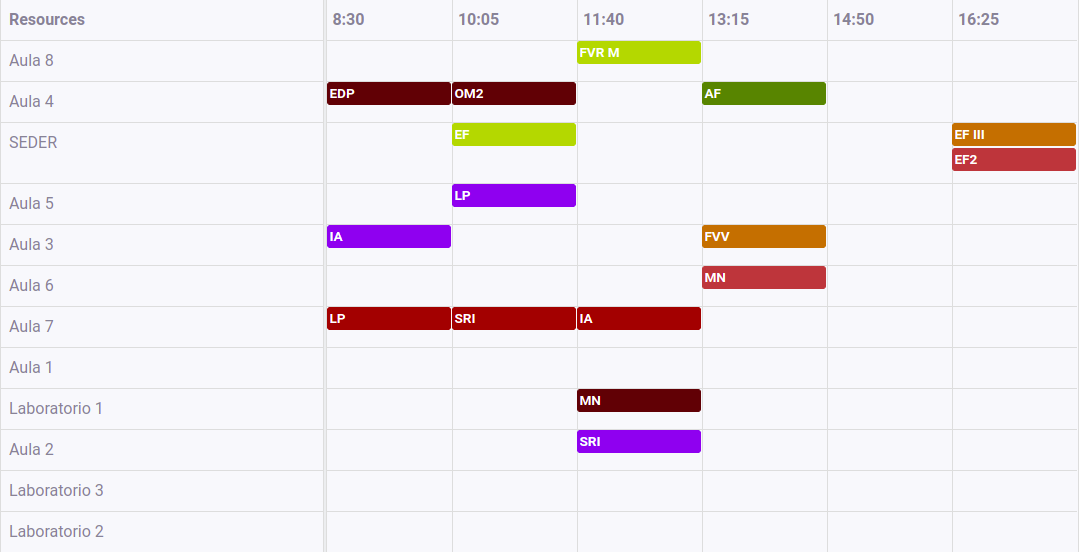
\includegraphics[width=0.95\linewidth]{images/Chapter 3/resource_distribution}
	\caption{Distribución por locales de los turnos de clase.}
	\label{fig:resource_distributions}
\end{figure}

\section{Autenticación}

La autenticación es una parte esencial en la mayoría de los sistemas y aplicaciones. Existen muchas formas y estrategias de manejar la misma. En el software que se presenta se pone en uso a través de un módulo independiente que posee todos los casos de uso y middlewares relacionados con tal aspecto. En esta ocasión el proceso se realiza por medio de JSON Web Token(JWT).

JWT es un estándar de internet propuesto para la creación de firmas y/o encriptación (opcional), cuyo contenido es enviado en forma de cadena de texto de backend a frontend (y viceversa), comunmente llamado \textit{token}.

\begin{figure}[h!]
	\centering
	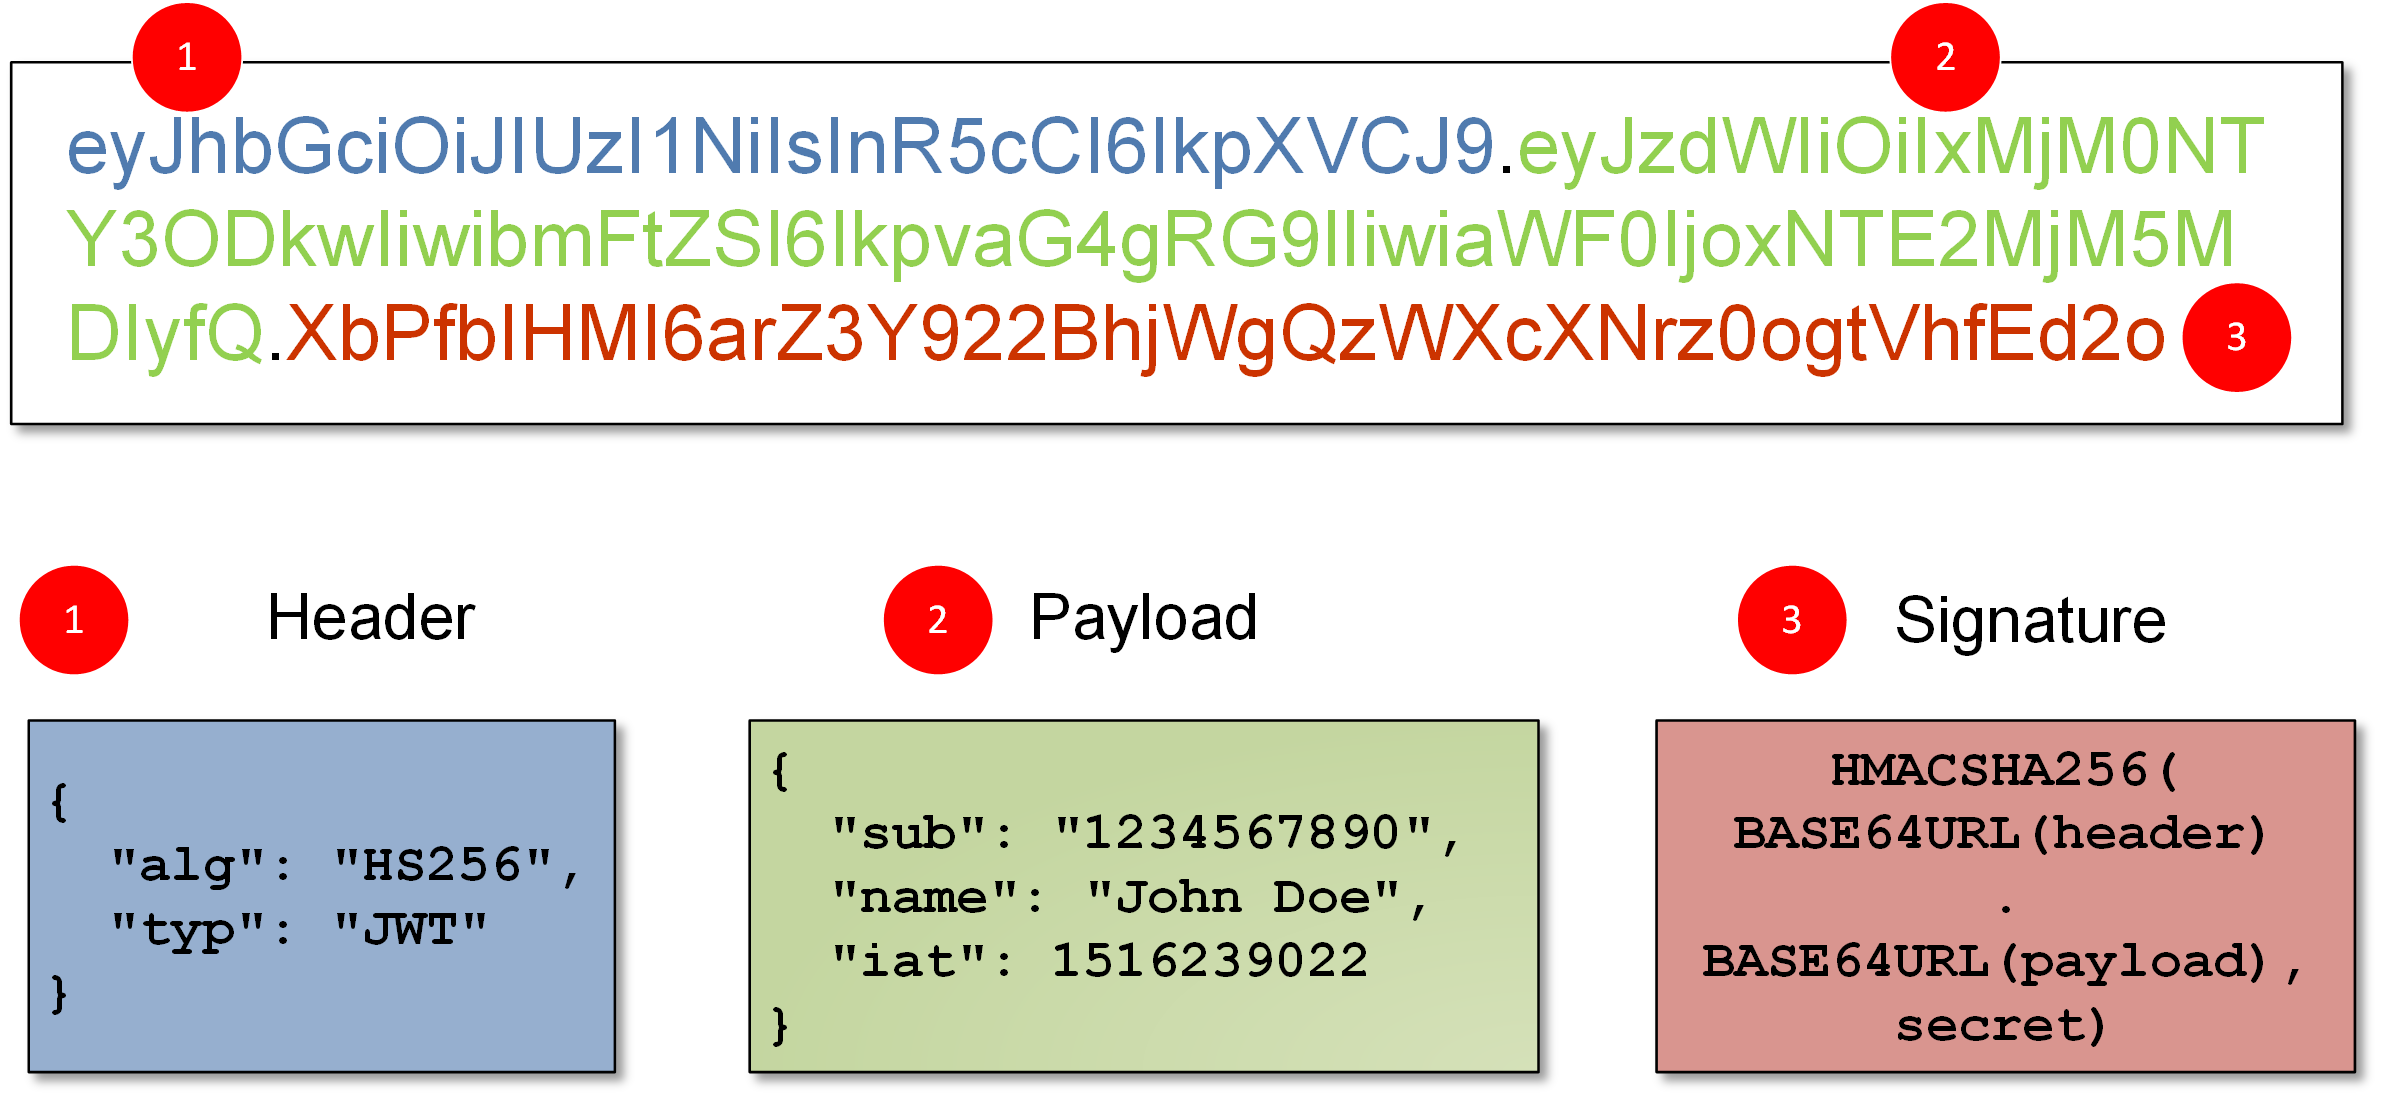
\includegraphics[width=0.95\linewidth]{images/Chapter 3/jwt1}
	\caption{Estructura del token \cite{jwt_image}}
	\label{fig:jwt}
\end{figure}

Cuando se recibe una petición de login por parte del cliente, el servidor se encarga de comprobar que las credenciales son correctas y la respuesta del login, es entre otras cosas, el token al que se hace referencia en el párrafo anterior. Supongamos después que se hace otra petición cliente-servidor y que el token se adjunta de forma apropiada en las cabeceras de la misma, cuando la petición arriba al punto adecuado, el servidor se encarga de ejecutar un \textit{middleware} (función intermedia) que procesa el token y verifica que sea el correcto, si todo este proceso se ejecuta sin mayores contratiempos, entonces en el request de la petición a través del campo user (request.user) se puede acceder al usuario que está intentado realizar la acción. En otro caso se responde con un estado 401 lo que indica que el usuario no esta autorizado al acceder al recurso que intenta solicitar. 

Todo este proceso antes descrito se realiza por medio de un paquete de terceros \textit{@nestjs/jwt} y además con la intervención de \textit{passport-jwt}



\section{Permisos y Usuarios}

En este sistema en particular los usuarios se clasifican en 2 grupos:

\begin{itemize}
	\item Los que solo pueden consultar el horario .
	\item Los que puede realizar acciones sobre algunas de sus entidades.
\end{itemize}

El primer grupo hace referencia a los usuario que solamente consultarán el sistema con el objetivo de estar al tanto de la información que se muestra en el mismo. Estos usuarios son considerados anónimos y por tanto solo podrán consumir los puntos de acceso que estén libres de permisos. Para ellos además se brindará la posibilidad de descargar el horario en formato Excel así como de estar al tanto de la felicidad del sistema.

El segundo grupo de usuario se separa, por otra parte, en dos conjuntos:

\begin{itemize}
	\item Profesores
	\item Usuarios administradores
\end{itemize}

A los profesores - previamente definidos por el administrador - se les dará la posibilidad de imponer sus propias restricciones (\ref{sec:restrictions}) sobre la distribución realizada e influir por en la felicidad final del sistema. Todas las demás utilidades están bloqueados para ellos.

Por otra parte, los administradores, son los que poseen todos los permisos; es decir, ellos tienen la potestad de modificar cualquier aspecto dentro del sistema; tanto de los turnos de clase como de las demás características relacionadas con la institución.

Los permisos son manejados por medio de un entero de 64 bits. Esto hace posible la optimización de espacio en la base de datos, así como la fácil representación de los mismos. Cada bit activo del número indica que el usuario \textit{X} puede realizar la acción correspondiente; luego para proceder al chequeo de estos, solo se hace necesario aplicar el operador binario \& (\ref{fig:and}) entre el entero que representa los permisos y el permiso en específico que se desea comprobar. Si el resultado de esta operación es mayor a 0, entonces el usuario puede completar la acción, en caso contrario se procede en consecuencia  y se responde negativamente al respecto.

\begin{figure}[h!]
	\centering
	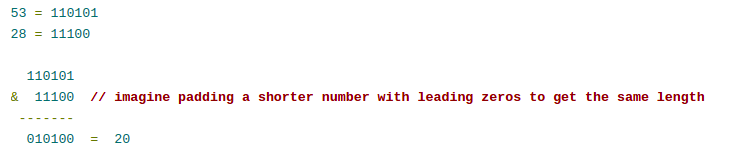
\includegraphics[width=0.95\linewidth]{images/Chapter 3/and}
	\caption{Operador \& entre dos números \cite{codeforces}}
	\label{fig:and}
\end{figure}

\noindent Luego activar un permiso para un usuario determinado no es más que: \\
\begin{equation}
	P \mid= (1 \ll p) \text{,}
\end{equation}

\noindent y para removerlo:\\
\begin{equation}
	\begin{split}	
		x & = \log_{2}(p \& -p) + 1  \\
		P & = P \& \sim(1 \ll (x - 1))
	\end{split}
\end{equation}

\noindent Donde se tiene que: \\
\begin{itemize}
	\item $P$: valor entero que representa los permisos que posee el usuario.
	\item $p$: permiso que se intenta adicionar o remover, según sea el caso.
\end{itemize}

Este enfoque ofrecido para los permisos, posee un inconveniente que no es muy difícil de notar: solamente se pueden representar 64 permisos en el sistema. En el software que se presenta, 64 permisos son más que suficientes para  gestionar todas las necesidades del mismo.

\section{Sistema de reportes}

Contar con una fácil distribución del contenido de manera offline, es un aspecto de notable importancia en muchos sistemas. En el que se propone, esta opción también se encuentra habilitada. 

Existe un módulo dedicado a cumplir esta tarea. La librería de NPM (Node Package Module) \texttt{excel4node}\cite{excel4node_npm}, es la encargada de gestionar e intervenir en todos los aspectos relacionados con la generación de un fichero en formato \textit{Excel} para asegurar cumplido el objetivo. Son innumerables las bondades que ofrece la misma, así como la facilidad para el trabajo con este tipo de ficheros, por tales motivos no trajo mayores dificultades considerar la utilización de esta en el desarrollo del software.

\section{Base de datos}

La base de datos que se utiliza para gestionar todo lo relacionado con la aplicación es \textit{PostgreSQL}; este es uno de los servidores de bases de datos más conocidos y utilizados a día de hoy. Está desarrollado bajo código abierto, razón por la que posee una gran comunidad que se encarga de trabajar en nuevas características constantemente. 

Existen varias razones que hacen que PostgreSQL resulte llamativo y que, por tanto, llevaron a su elección para este proyecto.
\begin{itemize}
	\item Multiplataforma: Se encuentra disponible en todas las versiones de los sistemas operativos Windows, Linux y Mac.
	\item Alto volumen: Ofrece un gran rendimiento cuando se hace necesario trabajar con grades volúmenes de información. Gracias al método de \textit{Control de Concurrencias Multiversión} se consigue un mejor performance cuando hay muchos movimientos dentro de la base de datos.
	\item Facilidad de manejo.
	\item Seguridad de la información: Hot-Standby es una de las cualidades más interesantes de Postgres. Hot-Standby permite que los usuarios puedan acceder a las tablas en modo lectura mientras que se realizan los procesos de backup o mantenimiento.
	\item \texttt{Tipos de datos}: Tiene soporte para tipos de datos avanzados tales como: arrays, hstore y tipos definidos por el usuario.
\end{itemize}

\section{Docker} 


Docker es una plataforma de código abierto para el desarrollo, manejo y ejecución de aplicaciones. Ofrece la ventaja de separar las aplicaciones de la infraestructura, por tal razón el despliegue de los sistemas se puede realizar relativamente rápido. Con el uso de docker  la infraestructura se maneja de la misma manera que se hace con las aplicaciones. Hablando de ventajas, las metodologías de docker para despliegue, integración y pruebas hacen que se reduzca significativamente el tiempo entre la escritura del código y el despliegue en producción del mismo. Además provee la habilidad de empaquetar y correr una aplicación en un ambiente aislado llamado \textit{contenedor}. Debido a este aislamiento y a la seguridad que ofrece se permite ejecutar varias aplicaciones simultaneamente en un servidor. Los contenedores son ligeros y contienen todo lo necesario para correr la aplicación, de esta forma, no es necesario preocuparse por lo que el serividor necesite instalar para su funcionamiento. Se puede compartir un contenedor mientras se está desarrollando  un proyecto y se garantiza que culaquiera que ejecute el mismo contenedor contendrá exactamente el mismo ambiente de trabajo que el desarrollador inicial.\cite{docker_dfn}

El sistema que se ofrece se encuentra desarrollado completamente sobre docker, tanto el frontend (que se despliega sobre nginx) como el backend (que se despliega sobre node). Esta integración hará que resulte de gran facilidad la instalación del software sobre cualquier red y que por tanto su pase a producción se realice sin mayores complicaciones. 

Las imágenes manejadas dentro del sistema están descritas en el siguiente enumerado; todas están disponibles en \href{https://hub.docker.com/}{\textit{Docker Hub}}:
\begin{itemize}
	\item node:16-alpine
	\item postgis/postgis:13-3.1-alpine
	\item adminer:latest
	\item nginx
\end{itemize}

El uso de ngnix será descrito en la siguiente sección.

\subsection{NGINX}

Nginx server es un servidor web gratuito y de código abierto. Se ejecuta en sistemas operativos Linux/Unix de 64 bits y es ampliamente utilizado para sitios web de alto rendimiento debido a su arquitectura liviana en comparación con otros servidores de la misma clase.

La herramienta fue incluida en este proyecto por medio de una imagen de Docker; e hizo posible que el frontend se desplegara a través de un servidor que se encargara de gestionar todos los temas de performance y manejo de peticiones.

Nginx fue lanzado oficialmente en octubre del 2004. El creador del software, Igor Sysoev, comenzó su proyecto en el 2002 como un intento de solucionar el problema C10k (reto de gestionar diez mil conexiones al mismo tiempo). Hoy en día, los servidores web tienen que manejar un número aún mas grande de conexiones. Por esa razón, Nginx ofrece una arquitectura asíncrona y controlada por eventos, característica que hace de él uno de los servidores más confiables para la velocidad y la escalabilidad. Muchos sitios web de alto tráfico usan el servicio, algunos de estos gigantes del internet son Google, Netflix, Adobe, Cloudflare, WordPress.com por solo mencionar algunos. \cite{nginx}


